%%%%% Preamble %%%%%
\documentclass[compress]{beamer} 
\usetheme{Madrid} 
\useoutertheme[subsection=false]{smoothbars} 
\useinnertheme{circles}
%%%%% Load Packages %%%%%
\usepackage{pgf}
\usepackage{endnotes}
\usepackage{natbib}
\usepackage{booktabs}
\usepackage{tikz}
\usetikzlibrary{shapes,arrows,positioning}
\usepackage{caption}
\captionsetup[figure]{labelformat=empty}
%%%%%%%%%%%%%%  Notes Options  %%%%%%%%%%%%%%%%%%%%%%%%%%%%%
\setbeameroption{hide notes} % Only slides
%\setbeameroption{show only notes} % Only notes
%\setbeameroption{show notes on second screen=right} % Both
%%%%%%%%%%%%%%%%%%%%%%%%%%%%%%%%%%%%%%%%%%%%%%%%%%
%%%%% Define Colors %%%%%
\definecolor{COLOR01}{RGB}{0,0,153} %PSUblue
\definecolor{COLOR02}{RGB}{204,204,204} %grey80
%%%%% Set Colors %%%%% 
\setbeamercolor*{normal text}{fg=black,bg=white}
\setbeamercolor*{alerted text}{fg=navy}
\setbeamercolor*{example text}{fg=black}
\setbeamercolor*{structure}{fg=COLOR01, bg=white}
\setbeamercolor*{palette primary}{fg=white,bg=COLOR01}
\setbeamercolor*{palette secondary}{fg=black,bg= COLOR02}
\setbeamercolor*{palette tertiary}{fg=white,bg=COLOR01}
\setbeamercolor*{palette quaternary}{fg=white,bg=COLOR01}
\setbeamercolor{titlelike}{fg=black, bg=COLOR02}
\setbeamercolor{frametitle}{fg=white, bg=COLOR01}
\setbeamercolor{frametitle right}{fg=white, bg=COLOR01}
\setbeamercolor{sidebar}{bg= COLOR01}
\setbeamercolor*{palette sidebar primary}{fg=white,bg=COLOR01}
\setbeamercolor*{palette sidebar secondary}{fg=white,bg=COLOR01}
\setbeamercolor*{palette sidebar tertiary}{fg=white,bg=COLOR01}
\setbeamercolor*{palette sidebar quaternary}{fg=white,bg=COLOR01}
\setbeamercolor*{item projected}{fg=black,bg=black!20}
\setbeamercolor{block title}{fg=black,bg=COLOR02}
\setbeamercolor{block title alerted}{use=alerted text,fg=white,bg=alerted text.fg!75!black}
\setbeamercolor{block title example}{use=example text,fg=white,bg=example text.fg!75!black}
\setbeamercolor{block body}{parent=normal text,use=block title,bg=block title.bg!15!bg}
\setbeamercolor{block body alerted}{parent=normal text,use=block title alerted,bg=block title alerted.bg!15!bg}
\setbeamercolor{block body example}{parent=normal text,use=block title example,bg=block title example.bg!15!bg}
\definecolor{grey50}{RGB}{127,127,127} 
\definecolor{grey30}{RGB}{77,77,77} 
\definecolor{navy}{RGB}{0,0,128} 
\usepackage{environ}% Requinavy for \NewEnviron, i.e. to read the whole body of the environment
\makeatletter
\newcounter{acolumn}%  Number of current column
\newlength{\acolumnmaxheight}%   Maximum column height
% `column` replacement to measure height
\newenvironment{@acolumn}[1]{%
    \stepcounter{acolumn}%
    \begin{lrbox}{\@tempboxa}%
    \begin{minipage}{#1}%
}{%
    \end{minipage}
    \end{lrbox}
    \@tempdimc=\dimexpr\ht\@tempboxa+\dp\@tempboxa\relax
    % Save height of this column:
    \expandafter\xdef\csname acolumn@height@\roman{acolumn}\endcsname{\the\@tempdimc}%
    % Save maximum height
    \ifdim\@tempdimc>\acolumnmaxheight
        \global\acolumnmaxheight=\@tempdimc
    \fi
}

% `column` wrapper which sets the height beforehand
\newenvironment{@@acolumn}[1]{%
    \stepcounter{acolumn}%
    % The \autoheight macro contains a \vspace macro with the maximum height minus the natural column height
    \edef\autoheight{\noexpand\vspace*{\dimexpr\acolumnmaxheight-\csname acolumn@height@\roman{acolumn}\endcsname\relax}}%
    % Call original `column`:
    \orig@column{#1}%
}{%
    \endorig@column
}

% Save orignal `column` environment away
\let\orig@column\column
\let\endorig@column\endcolumn

% `columns` variant with automatic height adjustment
\NewEnviron{acolumns}[1][]{%
    % Init vars:
    \setcounter{acolumn}{0}%
    \setlength{\acolumnmaxheight}{0pt}%
    \def\autoheight{\vspace*{0pt}}%
    % Set `column` environment to special measuring environment
    \let\column\@acolumn
    \let\endcolumn\end@acolumn
    \BODY% measure heights
    % Reset counter for second processing round
    \setcounter{acolumn}{0}%
    % Set `column` environment to wrapper
    \let\column\@@acolumn
    \let\endcolumn\end@@acolumn
    % Finally process columns now for real
    \begin{columns}[#1]%
        \BODY
    \end{columns}%
}
\makeatother
%DO NOT DELETE ANYTHING BEFORE THIS LINE RIGHT HERE % % % % % % % % % % % % % % % % % % % % % % % % % % % %
%EVERYTHING ABOVE HERE IS IMPORTANT AND WILL FUCK UP YOUR SLIDESHOW IF YOU DELETE IT % % % % % % % % % % % %
\title[Measuring Judicial Independence]{{\large Measuring Judicial Independence in the American States:}}
\subtitle{A Latent Variable Approach}

\author{Jeremy R. Johnson}
\institute[PSU]{The Pennylvania State University

\medskip
\textit{Jeremy.Johnson@PSU.edu}
}
\date{April 23, 2015} %Compile This on the Day of the Presentation % % % % % % % % % % % %

\begin{document}
% % % % % % % % % % % % % % % % % % % % % % %
\begin{frame}
\setbeamertemplate{headline}{}
\titlepage
\end{frame}
% % % % % % % % % % % % % % % % % % % % % %
\section{Theory}
\subsection{Defining Judicial Independence}
\begin{frame}{Defining Judicial Independence}
\only{ ``We all know what it means, yet frequently we advance arguments about `judicial independence' without articulating precisely what it means.'' - \cite{Becker1970}}<1>

\only{`` Judicial independence is merely the other side of the coin from judicial accountability'' -- \citep{Burbank2008}}<2>

	
\end{frame}
%%%%%%%%%%%%%%%%%%%%%%%%%%%%%%%%%%%%%%%%%%%%%%%%%%%%%%
\subsection{The Judicial Independence Continuum}
\begin{frame}{The Judicial Independence Continuum}
		\begin{figure}[tb]\centering\caption*{\textbf{Judicial Independence Continuum}}\label{IndCon}
		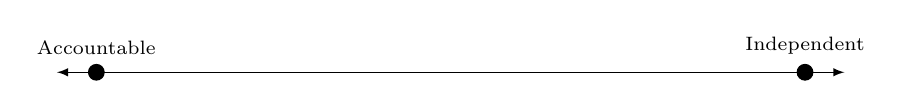
\begin{tikzpicture}
		% a straight line segment
		\draw[latex-latex] (-0.5,0) -- (9.5,0);
		%% the labels
		\node[fill=black,draw=black,circle,inner sep=2pt,label=above:{\scriptsize Independent}] at (9,0) {};
		\node[fill=black,draw=black,circle,inner sep=2pt,label=above:{\scriptsize Accountable}] at (0,0) {};
		\end{tikzpicture}
	\end{figure}
\end{frame}
%%%%%%%%%%%%%%%%%%%%%%%%%%%%%%%%%%%%%%%%%%%%%%%%%%%%%%%
\section{Indicators}
\begin{frame}{Indicators of Judicial Independence}
	\begin{itemize}
		\item Selection System
		\item Retention Election
		\item Term Length -- Inital and Subsequent
		\item Docket Control
	\end{itemize}
\end{frame}
%%%%%%%%%%%%%%%%%%%%%%%%%%%%%%%%%%%%%%%%%%%%%%%%%%%%%%
\subsection{Selection System}
\begin{frame}{Selection System}
\begin{figure}[tbh]\centering\caption{Selection Method Independence Continuum}\label{selectioncontinuum}
	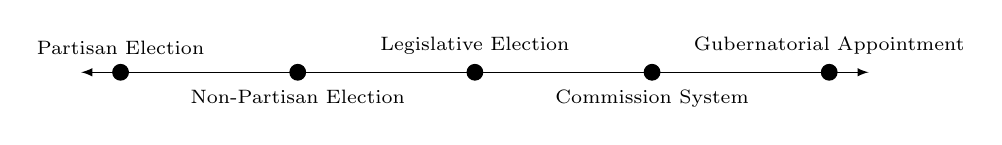
\begin{tikzpicture}
	% a straight line segment
	\draw[latex-latex] (-0.5,0) -- (9.5,0);
	%% the labels
	\node[fill=black,draw=black,circle,inner sep=2pt,label=above:{\scriptsize Gubernatorial Appointment}] at (9,0) {};
	\node[fill=black,draw=black,circle,inner
	sep=2pt,label=below:{\scriptsize Commission System}] at (6.75,0) {};
	\node[fill=black,draw=black,circle,inner
	sep=2pt,label=above:{\scriptsize Legislative Election}] at (4.5,0) {};
	\node[fill=black,draw=black,circle,inner
	sep=2pt,label=below:{\scriptsize Non-Partisan Election}] at (2.25,0) {};
	\node[fill=black,draw=black,circle,inner sep=2pt,label=above:{\scriptsize Partisan Election}] at (0,0) {};
	\end{tikzpicture}
\end{figure} 	
\end{frame}
%%%%%%%%%%%%%%%%%%%%%%%%%%%%%%%%%%%%%%%%%%%%%%%%%%%%%
\subsection{Retention Elections}
\begin{frame}{Retention Elections}
	\begin{figure}[tbh]\centering\caption{Retention Method Independence Continuum}\label{retentioncontinuum}
		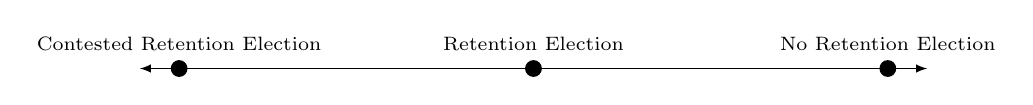
\begin{tikzpicture}
		% a straight line segment
		\draw[latex-latex] (-0.5,0) -- (9.5,0);
		%% the labels
		\node[fill=black,draw=black,circle,inner sep=2pt,label=above:{\scriptsize No Retention Election}] at (9,0) {};
		\node[fill=black,draw=black,circle,inner
		sep=2pt, label=above:{\scriptsize Retention Election}] at (4.5,0) {};
		\node[fill=black,draw=black,circle,inner sep=2pt,label=above:{\scriptsize Contested Retention Election}] at (0,0) {};
		\end{tikzpicture}
	\end{figure}	
\end{frame}
%%%%%%%%%%%%%%%%%%%%%%%%%%%%%%%%%%%%%%%%%%%%%%%%%%%%%%
\subsection{Term Length}
\begin{frame}{Term Length}
\begin{figure}[tbh]\centering\caption{Term Length Independence Continuum}\label{termcontinuum}
	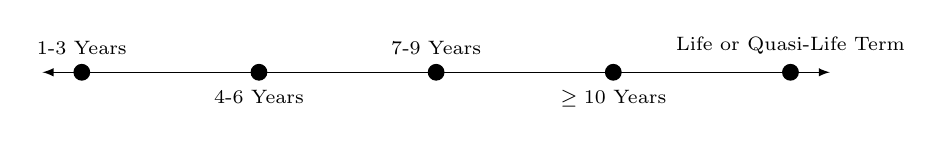
\begin{tikzpicture}
	% a straight line segment
	\draw[latex-latex] (-0.5,0) -- (9.5,0);
	%% the labels
	\node[fill=black,draw=black,circle,inner sep=2pt,label=above:{\scriptsize Life or Quasi-Life Term}] at (9,0) {};
	\node[fill=black,draw=black,circle,inner
	sep=2pt,label=below:{\scriptsize $\geq10$ Years}] at (6.75,0) {};
	\node[fill=black,draw=black,circle,inner
	sep=2pt,label=above:{\scriptsize 7-9 Years}] at (4.5,0) {};
	\node[fill=black,draw=black,circle,inner
	sep=2pt,label=below:{\scriptsize 4-6 Years}] at (2.25,0) {};
	\node[fill=black,draw=black,circle,inner sep=2pt,label=above:{\scriptsize 1-3 Years}] at (0,0) {};
	\end{tikzpicture}	
\end{figure}	
\end{frame}
%%%%%%%%%%%%%%%%%%%%%%%%%%%%%%%%%%%%%%%%%%%%%%%%%%%%%%%%%%%%%%
\subsection{Docket Control}
\begin{frame}{Docket Control}
\begin{figure}[tbh]\centering\caption{Docket Control Independence Continuum}\label{docketcontinuum}
	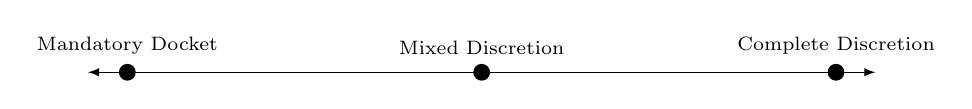
\begin{tikzpicture}
	% a straight line segment
	\draw[latex-latex] (-0.5,0) -- (9.5,0);
	%% the labels
	\node[fill=black,draw=black,circle,inner sep=2pt,label=above:{\scriptsize Complete Discretion}] at (9,0) {};
	\node[fill=black,draw=black,circle,inner
	sep=2pt,label=above:{\scriptsize Mixed Discretion}] at (4.5,0) {};
	\node[fill=black,draw=black,circle,inner sep=2pt,label=above:{\scriptsize Mandatory Docket}] at (0,0) {};
	\end{tikzpicture}
\end{figure}	
\end{frame}
%%%%%%%%%%%%%%%%%%%%%%%%%%%%%%%%%%%%%%%%%%%%%%%%%%%%%%%
\section{Model}
\subsection{Specification}
\begin{frame}{Specification}
	\begin{itemize}
		\item Bayesian IRT Model
		\item 4 or 5 Indicators
	\end{itemize}
\end{frame}
%%%%%%%%%%%%%%%%%%%%%%%%%%%%%%%%%%%%%%%%%%%%%%%%%%%%%%
\subsection{Model}
\begin{frame}{Model}
	\only{Probability Distribution for a Given Response}<1>
	\only{\begin{align*}
	P[y_{ij}=k]=F(\alpha_{jk}-\theta_{it}\beta_j)-F(\alpha_{jk-1}-\theta_{it}\beta_j)
	\end{align*}}<1>
\end{frame}
%%%%%%%%%%%%%%%%%%%%%%%%%%%%%%%%%%%%%%%%%%%%%%%%%%%%%%%
\subsection{Model}
\begin{frame}{Model}
	\only{Liklihood for Logistic Distribution}<2>
	\only{\begin{align*}
		{\cal L} (\beta,\alpha,\theta|y)=\prod_{i=1}^{N}\prod_{t=1}^{T}\prod_{j=1}^{J}[F(\alpha_{jy_{itj}}-\theta_{it}\beta_j)-F(\alpha_{jy_{itj}-1}-\theta_{it}\beta_j)]
		\end{align*} }<2>
\end{frame}
%%%%%%%%%%%%%%%%%%%%%%%%%%%%%%%%%%%%%%%%%%%%%%%%%%%%%
\section{Results}
\subsection{Five Indicator Model}
\begin{frame}{Five Indicator Model Over Time}
\begin{figure}
\centering
\includegraphics[scale=.35]{graphics/fiveind/fiveind_timeplot}
\end{figure}
\end{frame}
%%%%%%%%%%%%%%%%%%%%%%%%%%%%%%%%%%%%%%%%%%%%%%%%%%%%%%
\subsection{Five Indicator Additive Model}
\begin{frame}{Five Indicator Additive Model}	
\begin{figure}\centering
\includegraphics[scale=.5]{graphics/fiveind/fiveind_additive_ggplot}
\caption{Pearson's $R=-.9553$ }
\end{figure}
\end{frame}
%%%%%%%%%%%%%%%%%%%%%%%%%%%%%%%%%%%%%%%%%%%%%%%%%%%%%%
\subsection{Five Indicator Betas}
\begin{frame}{Five Indicator Beta Discrimination}	
\begin{center}
\includegraphics[scale=.5]{graphics/fiveind/FiveBetaDiscrimination}
\end{center}
\end{frame}
%%%%%%%%%%%%%%%%%%%%%%%%%%%%%%%%%%%%%%%%%%%%%%%%%%%%%%%
\subsection{}
\begin{frame}{Judicial Independence Over Time}
\begin{center}
\includegraphics[scale=.5]{graphics/fiveind/meanavgtime}
\end{center}
\end{frame}
%%%%%%%%%%%%%%%%%%%%%%%%%%%%%%%%%%%%%%%%%%%%%%%%%%%%%%%%
\subsection{Regime Change Model}
\begin{frame}{Regime Change Model Scores}
	\begin{columns}[c]
		\column{1.5in}
		\begin{center}
			\includegraphics[scale=.3]{graphics/regime/regime_param_mean_first_ggplot}
		\end{center}
		\column{1.5in}
		\begin{center}
			\includegraphics[scale=.3]{graphics/regime/regime_param_mean_second_ggplot}
		\end{center}
	\end{columns}
\end{frame}
%%%%%%%%%%%%%%%%%%%%%%%%%%%%%%%%%%%%%%%%%%%%%%%%%%%%%%%
\subsection{Convergent Validity}
\begin{frame}{Convergent Validity-Ginsburg and Melton Replicaton}
	% latex table generated in R 3.1.2 by xtable 1.7-4 package
	% Fri Apr 17 11:58:40 2015
	\begin{table}[ht]
		\centering\caption*{Correlation of Measures}\label{Correlation}
		\begin{tabular}{rccc}
			\hline
			& Additive & IRT & \citeauthor{Melton2014} \\ 
			\hline
			Additive & -- & $-.95^{***}$ &$-0.45^{**}$ \\ 
			IRT & $-0.95^{***}$ & -- & $0.52^{***}$ \\ 
			\citeauthor{Melton2014} & $-0.45^{**}$  &  $0.52^{***}$ & --\\ 
			\hline
			\textit{Note:}  & \multicolumn{3}{l}{$^{*}$p$<$0.1; $^{**}$p$<$0.05; $^{***}$p$<$0.01} \\
		\end{tabular}
	\end{table}
\end{frame}
%%%%%%%%%%%%%%%%%%%%%%%%%%%%%%%%%%%%%%%%%%%%%%%%%%%%%%
\subsection{Discriminant Validity}
\begin{frame}{Random Measures Replication}
	% latex table generated in R 3.1.2 by xtable 1.7-4 package
	% Fri Apr 17 20:25:11 2015
	\begin{table}[ht]
		\centering\caption{Correlation of Estimates with \citet{Enns2013}}\label{EKCor}
		\begin{tabular}{rcccc}
			\hline
			&  Mood &  2 Dimension Mood & Posterior Estimates & Additive \\ 
			\hline
			Mood & -- & $0.58^{***}$ & $0.40^{**}$ & $-0.40^{**}$ \\ 
			2 Dimension Mood &  $0.58^{***}$ & -- & $0.16$ & $-0.15$ \\ 
			Posterior Estimates &  $0.40^{**}$  &  $0.16$  & -- & $-0.95^{***}$ \\ 
			Additive & $-0.40^{**}$  & $-0.15$  & $-0.95^{***}$ & -- \\ 
			\hline
			\textit{Note:}  & \multicolumn{4}{l}{$^{*}$p$<$0.1; $^{**}$p$<$0.05; $^{***}$p$<$0.01} \\
		\end{tabular}
	\end{table}
\end{frame}
%%%%%%%%%%%%%%%%%%%%%%%%%%%%%%%%%%%%%%%%%%%%%%%%%%%%%%%
\begin{frame}{Questions?}
	
\end{frame}
%%%%%%%%%%%%%%%%%%%%%%%%%%%%%%%%%%%%%%%%%%%%%%%%%%%%%%%
\newpage
\appendix
\section*{References}
\begin{frame}{References}
\bibliographystyle{apsr}
\bibliography{measurementbib}
\end{frame}
\end{document}